
\RequirePackage{currfile} 
\documentclass{beamer}



%%%%%%%%%%%%%% PACKAGES %%%%%%%%%%%%%%%%%%%%%
\usepackage{textpos}   
\usepackage{graphicx} % Allows including images
\usepackage{booktabs} % Allows the use of \toprule, \midrule and \bottomrule in tables
\usepackage{biblatex} % Allows for \cite 
\usepackage[utf8]{inputenc}
\usepackage{tikz} \usetikzlibrary{calc, arrows.meta, intersections, patterns, positioning, shapes.misc, fadings, through,decorations.pathreplacing}
\usepackage{array} % To pause columns
\usepackage[usenames,dvipsnames]{xcolor}
\usepackage{colortbl}
\usepackage{multicol}
\usepackage{multirow}
\usepackage{caption}
\usepackage{block} %blocks for statements
\usepackage{comment}
\usepackage[absolute,overlay]{textpos}
\usepackage{forest}
\forestset{qtree/.style={for tree={parent anchor=south, 
           child anchor=north,align=center,inner sep=0pt}}}


\definecolor{ColorOne}{named}{MidnightBlue}
\definecolor{ColorTwo}{named}{Dandelion}
\definecolor{ColorThree}{named}{Plum}

\tikzstyle{descript} = [text = black,align=center, minimum height=1.8cm, align=center, outer sep=0pt,font = \footnotesize]
\tikzstyle{activity} =[align=center,outer sep=1pt]

%% Change the bg color to adjust your transition slide background color!
\newenvironment{transitionframe}{
  \setbeamercolor{background canvas}{bg=White}
  \begin{frame}}{
    \end{frame}
}

%%%%%%%%%%%%%% COMMANDS %%%%%%%%%%%%%%%%%%%%%
\newcommand{\progressbar}{%
\pgfmathsetmacro{\theta}{360/\inserttotalframenumber*\insertframenumber}
\begin{tikzpicture}[scale=0.025]
\fill[blue] (0,0) circle (9);
\fill[green] (0,0) -- (9,0) arc (0:-\theta:9);
\fill[white] (0,0) circle (5);
\node at (0,0) {\insertframenumber};
\end{tikzpicture}
}

%%% TIKZ STUFF
\tikzset{   
        every picture/.style={remember picture,baseline},
        every node/.style={anchor=base,align=center,outer sep=1.5pt},
        every path/.style={thick},
        }
\newcommand\marktopleft[1]{%
    \tikz[overlay,remember picture] 
        \node (marker-#1-a) at (-.3em,.3em) {};%
}
\newcommand\markbottomright[2]{%
    \tikz[overlay,remember picture] 
        \node (marker-#1-b) at (0em,0em) {};%
}
\tikzstyle{every picture}+=[remember picture] 
\tikzstyle{mybox} =[draw=black, very thick, rectangle, inner sep=10pt, inner ysep=20pt]
\tikzstyle{fancytitle} =[draw=black,fill=red, text=white]
%%%% END TIKZ STUFF

%%% COLOR COLUMN (did not make it work...)
\newcolumntype{G}{>{\centering\columncolor{gray!20!white}}p{0.2\textwidth}}
\newcolumntype{C}{>{\centering\arraybackslash}p{0.2\textwidth}}
%%% END COLOR COLUMN


\AtBeginSection[]{
  \begin{frame}
  \vfill
  \centering
  \begin{beamercolorbox}[sep=8pt,center,shadow=true,rounded=true]{title}
    \usebeamerfont{title}\insertsectionhead\par%
  \end{beamercolorbox}
  \vfill
  \end{frame}
}

%%%%%%%%%%%%%%% SETTINGS %%%%%%%%%%%%%%%%%%%%%%%
\mode<presentation> {
%\usetheme{Warsaw}
%\usetheme{Frankfurt}
%\usetheme{Madrid}
\usetheme{default}
%\usecolortheme{whale}
\usecolortheme{default}
\usefonttheme{professionalfonts}
}

%To call references
%\bibliographystyle{../aea.bst}
%\bibliography{references}

%%%%%%%%%%%%%%%%%%%%%%%%%%%%%%%%%%
%FOR LINKS
\definecolor{darkblue}{rgb}{0.0, 0.0, 0.65}
\definecolor{darkgreen}{rgb}{0.0, 0.65, 0.0}
\hypersetup{
	citecolor=blue,
	colorlinks=true,
	linkcolor=blue,
	filecolor=magenta,
	urlcolor=magenta
}
%%%%%%%%%%%%%%%%%%%%%%%%%%%%%%%%%%


\setbeamertemplate{navigation symbols}{} 


%Title
\title[]{New Idea: School closures, remote learning and differential effects between only childs and children with siblings}
%\subtitle[]{DLP Writing Seminar}

\author[Francisco Pardo] % (optional, for multiple authors)
{Francisco Pardo - fpardo@utexas.edu \inst{1}}
 
\institute[UT] % (optional)
{
  \inst{1}%
  University of Texas at Austin
  %\and
  %\inst{2}%
   % ...
}

\date{\today}
 

 
 
%------------------------------------------------------------
%The next block of commands puts the table of contents at the 
%beginning of each section and highlights the current section:
%Commented because presentations are short, we don't need that. 
\begin{comment}
\AtBeginSection[]
{
  \begin{frame}
    \frametitle{Table of Contents}
    \tableofcontents[currentsection]
  \end{frame}
}
\end{comment}
%------------------------------------------------------------

\begin{document}


\frame{\titlepage}



\begin{frame}
   \frametitle{Motivation}
   \begin{itemize}
       \item School closures and remote learning had huge impacts on learning. 
       \item These were bigger in low SES schools.
       \item Some initial evidence that only childs and children with siblings might be affected differently by lockdowns and remote learning.
       \item Peru had school closures for 2 years.
       \item \textbf{Research Question: Who had a bigger negative impact, only children or children with siblings? Why?}
   \end{itemize}
\end{frame}


\begin{frame}
    \label{mccrary}
    \frametitle{Literature}
        {\resizebox{0.9\textwidth}{!}{
       
\includegraphics{./FIGURES/DLP/literature.png}
    }
  }  
\end{frame}

\begin{frame}
    \frametitle{Some potential channels}
    \begin{itemize}
        \item \textbf{Parental Attention:} Only children might have benefited from more focused parental attention.
        \item \textbf{Siblings as Support:} Only children may be more affected by lack of peers and loneliness.
        \item \textbf{Limited Resources:} Access to online classes might be more limited when having many siblings. Sharing a space and having them around may also be distracting.
    \end{itemize}
\end{frame}

\begin{frame}
    \frametitle{Contribution}
    \begin{itemize}
        \item Household education production process.
        \item Household spillovers
        \item Disaster and heterogeneous effects
    \end{itemize}
\end{frame}


\begin{frame}
    \frametitle{Empirical Strategy: Regression discontinuity}
    
    $Y_{itgs}=\alpha_{c} + \sum_{k=-5}^{-2}   \gamma_k D_{it} + \sum_{k=0}^{4} \beta_k D_{it} + D_{it}  + \tau_{t} + \phi_{g} + \delta_{s} + \mu{i} \epsilon_{itgs}$ 
   
    
    \bigskip \\
    $Y_{itgs}$: Outcome for student $i$ in year $t$ in grade $g$ and school $s$. \\
    $\tau_{t}$: year FE
    $\phi_{g}$: grade FE
    $\delta_{s}$: school FE
    $\mu_{i}$: Individual FE
    $D_{i} $: Child has siblings
    
\end{frame}

\begin{frame}
    \frametitle{Preliminary results}
    \begin{itemize}
        \item Students with siblings are significantly more affected by the COVID shock than only childs.
        \item Standardized GPA $\downarrow$ 0.04sd
        \item These are similar for urban/rural and parents w/wo higher education
        \item Here I show results from GPA of elementary school
        \item ~ 80mm observations so confidence intervals are quite small
    \end{itemize}
\end{frame}



\begin{frame}
    \label{overall_gpa}
    \frametitle{Reduction in Mathematics and Reading GPA}
        {\resizebox{0.9\textwidth}{!}{
       \includegraphics{./FIGURES/COVID/covid_ece_gpa_all_no_elm.png}
    }
  }  
\end{frame}


\begin{frame}
\frametitle{Admission scores relative to estimated admission cutoff}

\begin{columns}[T]
\begin{column}{.5\textwidth}
Urban
{\resizebox{\textwidth}{!}{
       \includegraphics{./FIGURES/COVID/covid_ece_gpa_urban_no_elm.png}
    }
  }

\end{column}
\hfill
\begin{column}{.5\textwidth}
Rural
{\resizebox{\textwidth}{!}{
       \includegraphics{./FIGURES/COVID/covid_ece_gpa_rural_no_elm.png}
    }
  }
\end{column}
\end{columns}
\end{frame}






\begin{frame}
    \label{ece_4p}
    \frametitle{GPA Elementary: Math and reading}
        {\resizebox{0.9\textwidth}{!}{
       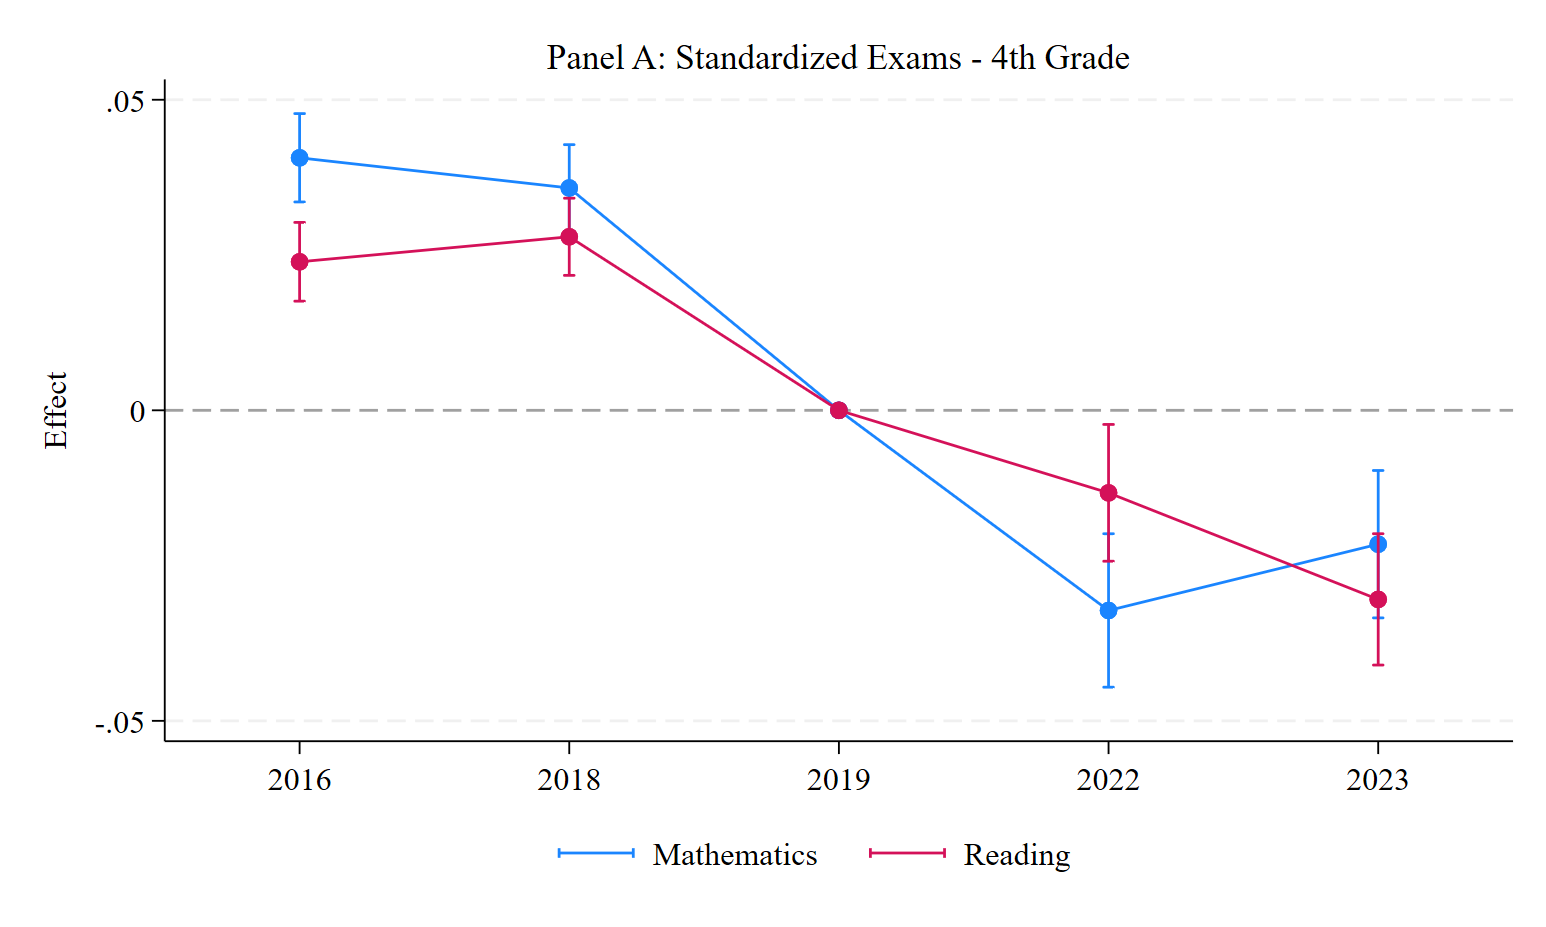
\includegraphics{./FIGURES/DLP/covid_ece_4p.png}
    }
  }  
\end{frame}







\begin{frame}
    \label{ece_4p}
    \frametitle{Standardized Test Scores: 4th grade}
        {\resizebox{0.9\textwidth}{!}{
       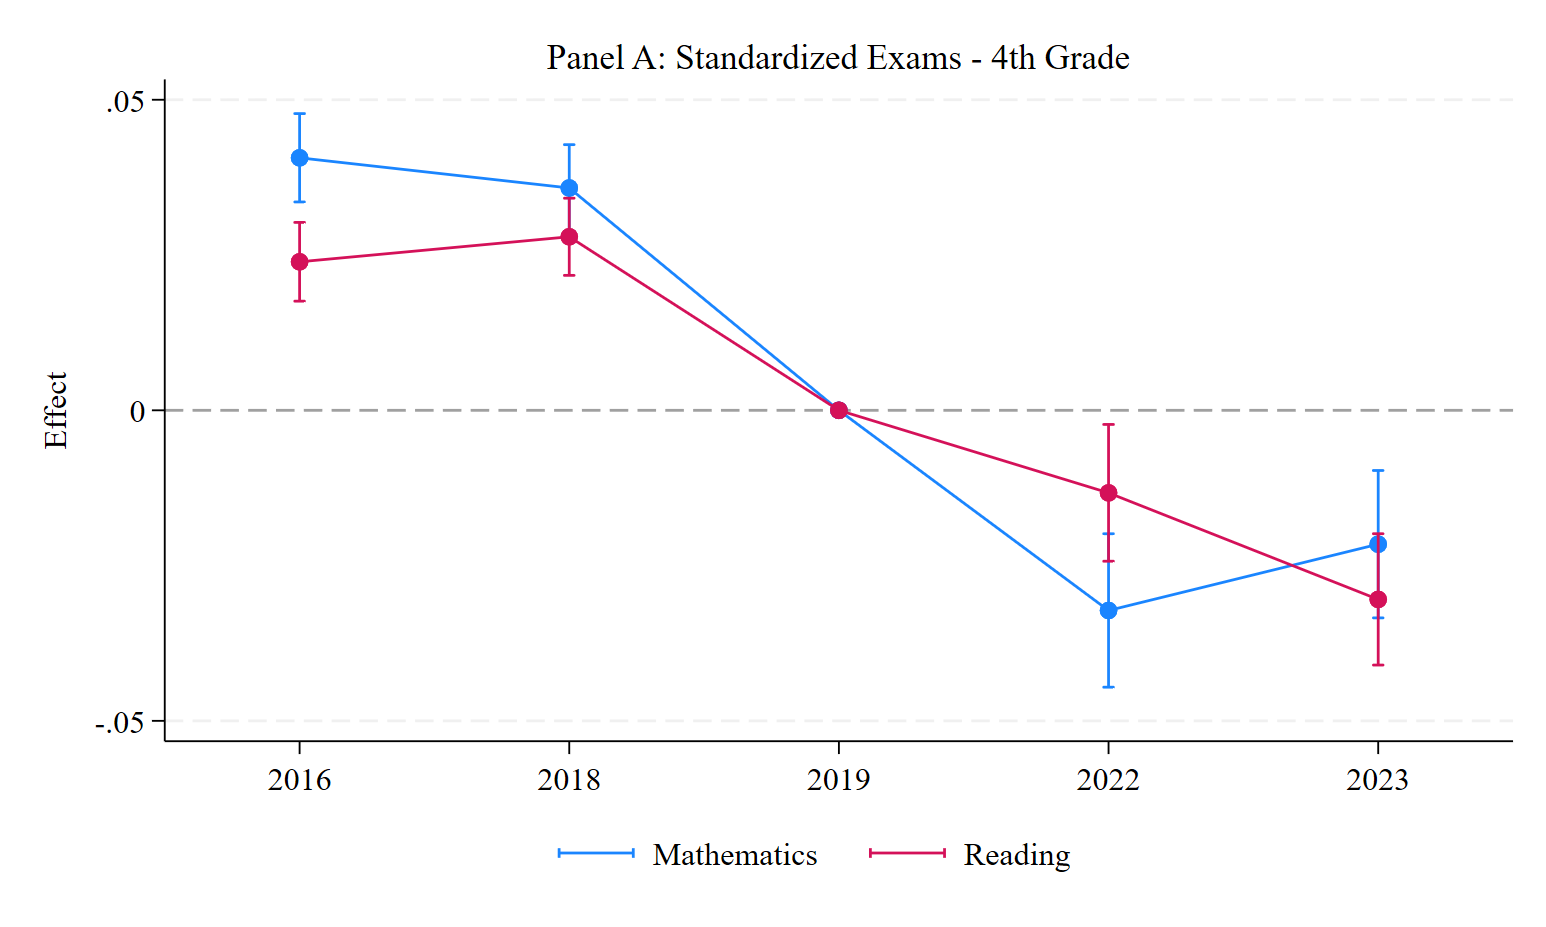
\includegraphics{./FIGURES/DLP/covid_ece_4p.png}
    }
  }  
\end{frame}

\begin{frame}
    \label{ece_2s}
    \frametitle{Standardized Test Scores: 8th grade}
        {\resizebox{0.9\textwidth}{!}{
       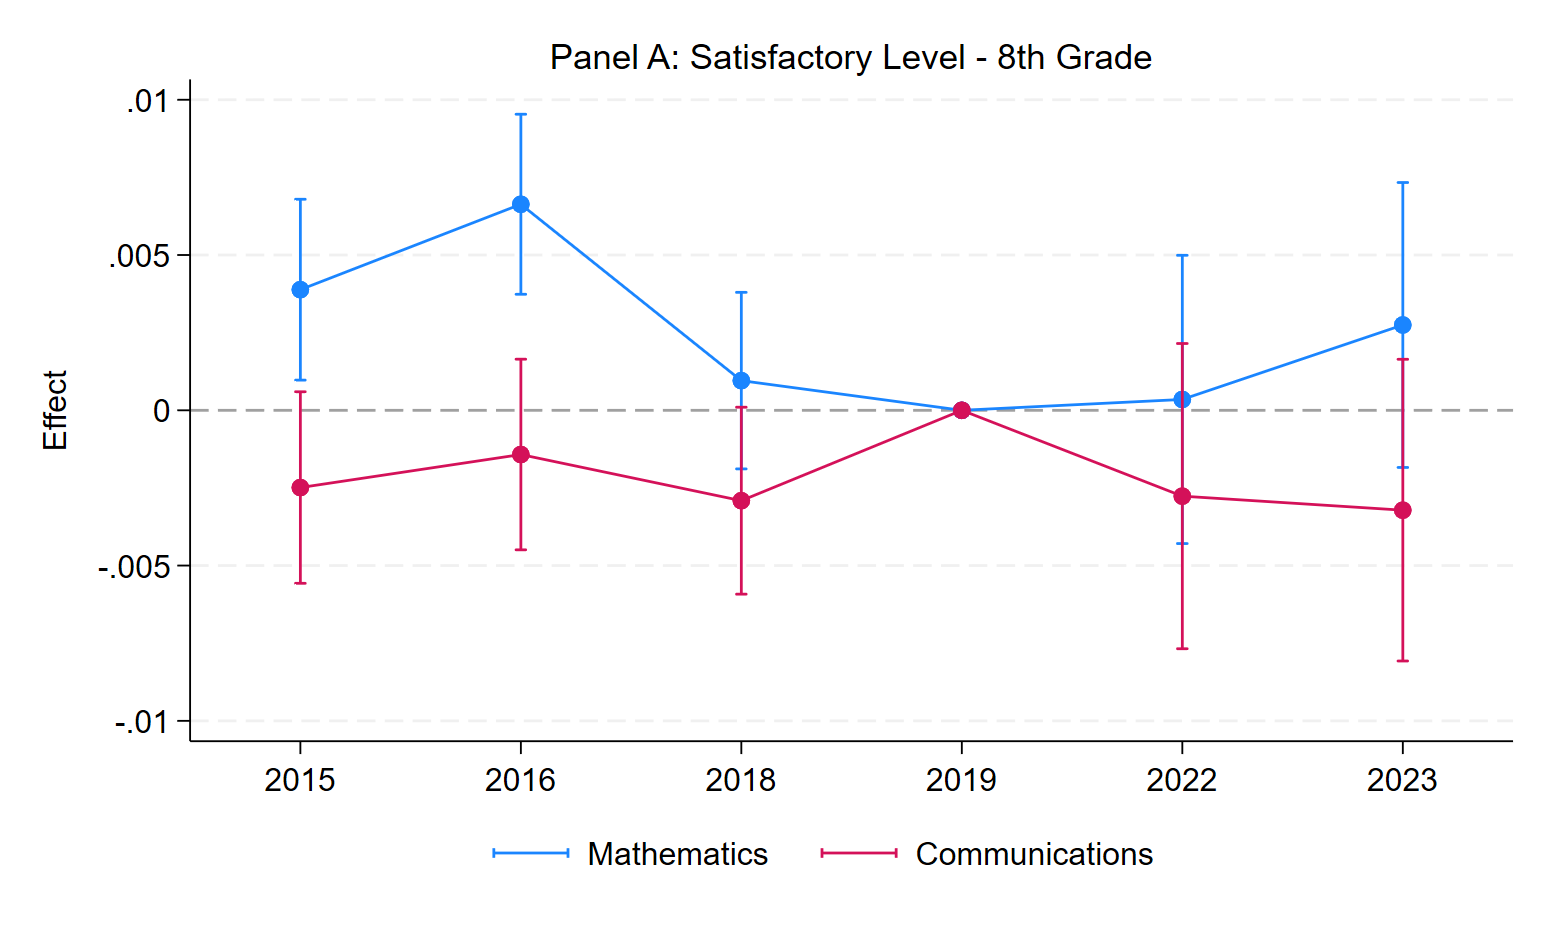
\includegraphics{./FIGURES/DLP/covid_ece_2s.png}
    }
  }  
\end{frame}


\begin{frame}
    \label{gpa}
    \frametitle{High-School GPA}
        {\resizebox{0.9\textwidth}{!}{
       \includegraphics{./FIGURES/DLP/covid_ece_gpa.png}
    }
  }  
\end{frame}

\begin{frame}
    \label{pass}
    \frametitle{Grade Pass Rate}
        {\resizebox{0.9\textwidth}{!}{
       \includegraphics{./FIGURES/DLP/covid_ece_approved.png}
    }
  }  
\end{frame}



\begin{section}
    {Main Results: Heterogeneous effects}
\end{section}


\begin{frame}
    \label{pass}
    \frametitle{Potential next steps}
       \begin{itemize}
           \item Resources in the household: Internet, computer, etc.
           \item 
           \item Other descriptive characteristics:
            \begin{itemize}
                \item  Use of time survey 2010 & 2024
                \item Emotional Well-being survey 6th grade, 2024.
            \end{itemize}
       \end{itemize}
    
\end{frame}


\end{document}
        



\end{document}
        